\section {Photonik}
\subsection {Grundlagen}
\subsubsection {Der Begriff Photonik}
Unter Photonik (englisch: photonics) wird die Gesamtheit der optischen Techniken verstanden, mit der Licht erzeugt, verstärkt, geformt, übertragen, gemessen und als elektromagnetische Strahlung nutzbar gemacht wird. Basis für diese neuen Werkzeuge aus Licht sind die klassische Optik, die Optoelektronik und Lasertechnik. Durch die fast grenzenlosen Einsatzmöglichkeiten ist Photonik zur Querschnitts-und Schlüsseltechnologie geworden. Die auch als optische Technologien bezeichneten Produkte werden in Autos, Computern, CD-Playern, Handys, Fernbedienungen, in der Kommunikationstechnik, beim Röntgen oder in der industriellen Fertigungstechnik eingesetzt. Kernprodukte wie Laser oder Glasfasern machen andere Innovationen erst möglich.

\subsection {Physikalische Grundlagen}
\subsubsection {Elektromagnetische Strahlung}
Licht ist der für das Auge sichtbare Teil der elektromagnetischen Strahlung. Im elektromagnetischen Spektrum umfasst der Bereich des Lichts Wellenlängen von etwa 380 nm bis 780 nm. Elektromagnetische Strahlung existiert aber in einem wesentlich grösseren Frequenzbereich. Nur ein kleiner Frequenzbereich ist für Menschen sichtbar.
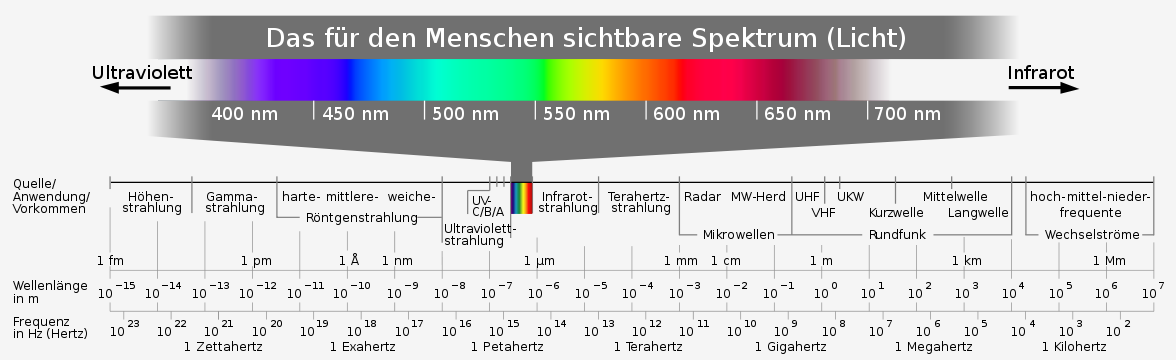
\includegraphics[width=\textwidth]{images/strahlung}

\begin{multicols}{2}
\paragraph {Lichtgeschwindigkeit im Vakuum}
$c = \frac {1}{\sqrt{\mu_0 \epsilon_0}} = 299792458 \frac{m}{s}$

\paragraph {Lichtgeschwindigkeit im Medium}
$c = \frac {1}{\sqrt{\mu_0 \mu_r \epsilon_0 \epsilon_r}}$ auf Leiterplatte $c = 20 \frac{cm}{ns}$ 
\end{multicols}

\paragraph {Photonen}
Licht besteht aus diskreten Energiequanten, den so genannten Photonen.
\begin{multicols}{3}
Energie: \\ $E = h * v$ \\
Plancksche Wirkungsquantum: \\ $h = 6.62606957 * 10^{-34} Js$ \\
Impuls: \\ $p = \frac {h}{\lambda}$ 
\end{multicols}